\documentclass{standalone}
\usepackage{tikz}
\usetikzlibrary{patterns, positioning}
\usepackage[sfdefault]{ClearSans} %% option 'sfdefault' activates Clear Sans as the default text font
\usepackage[T1]{fontenc}

\begin{document}
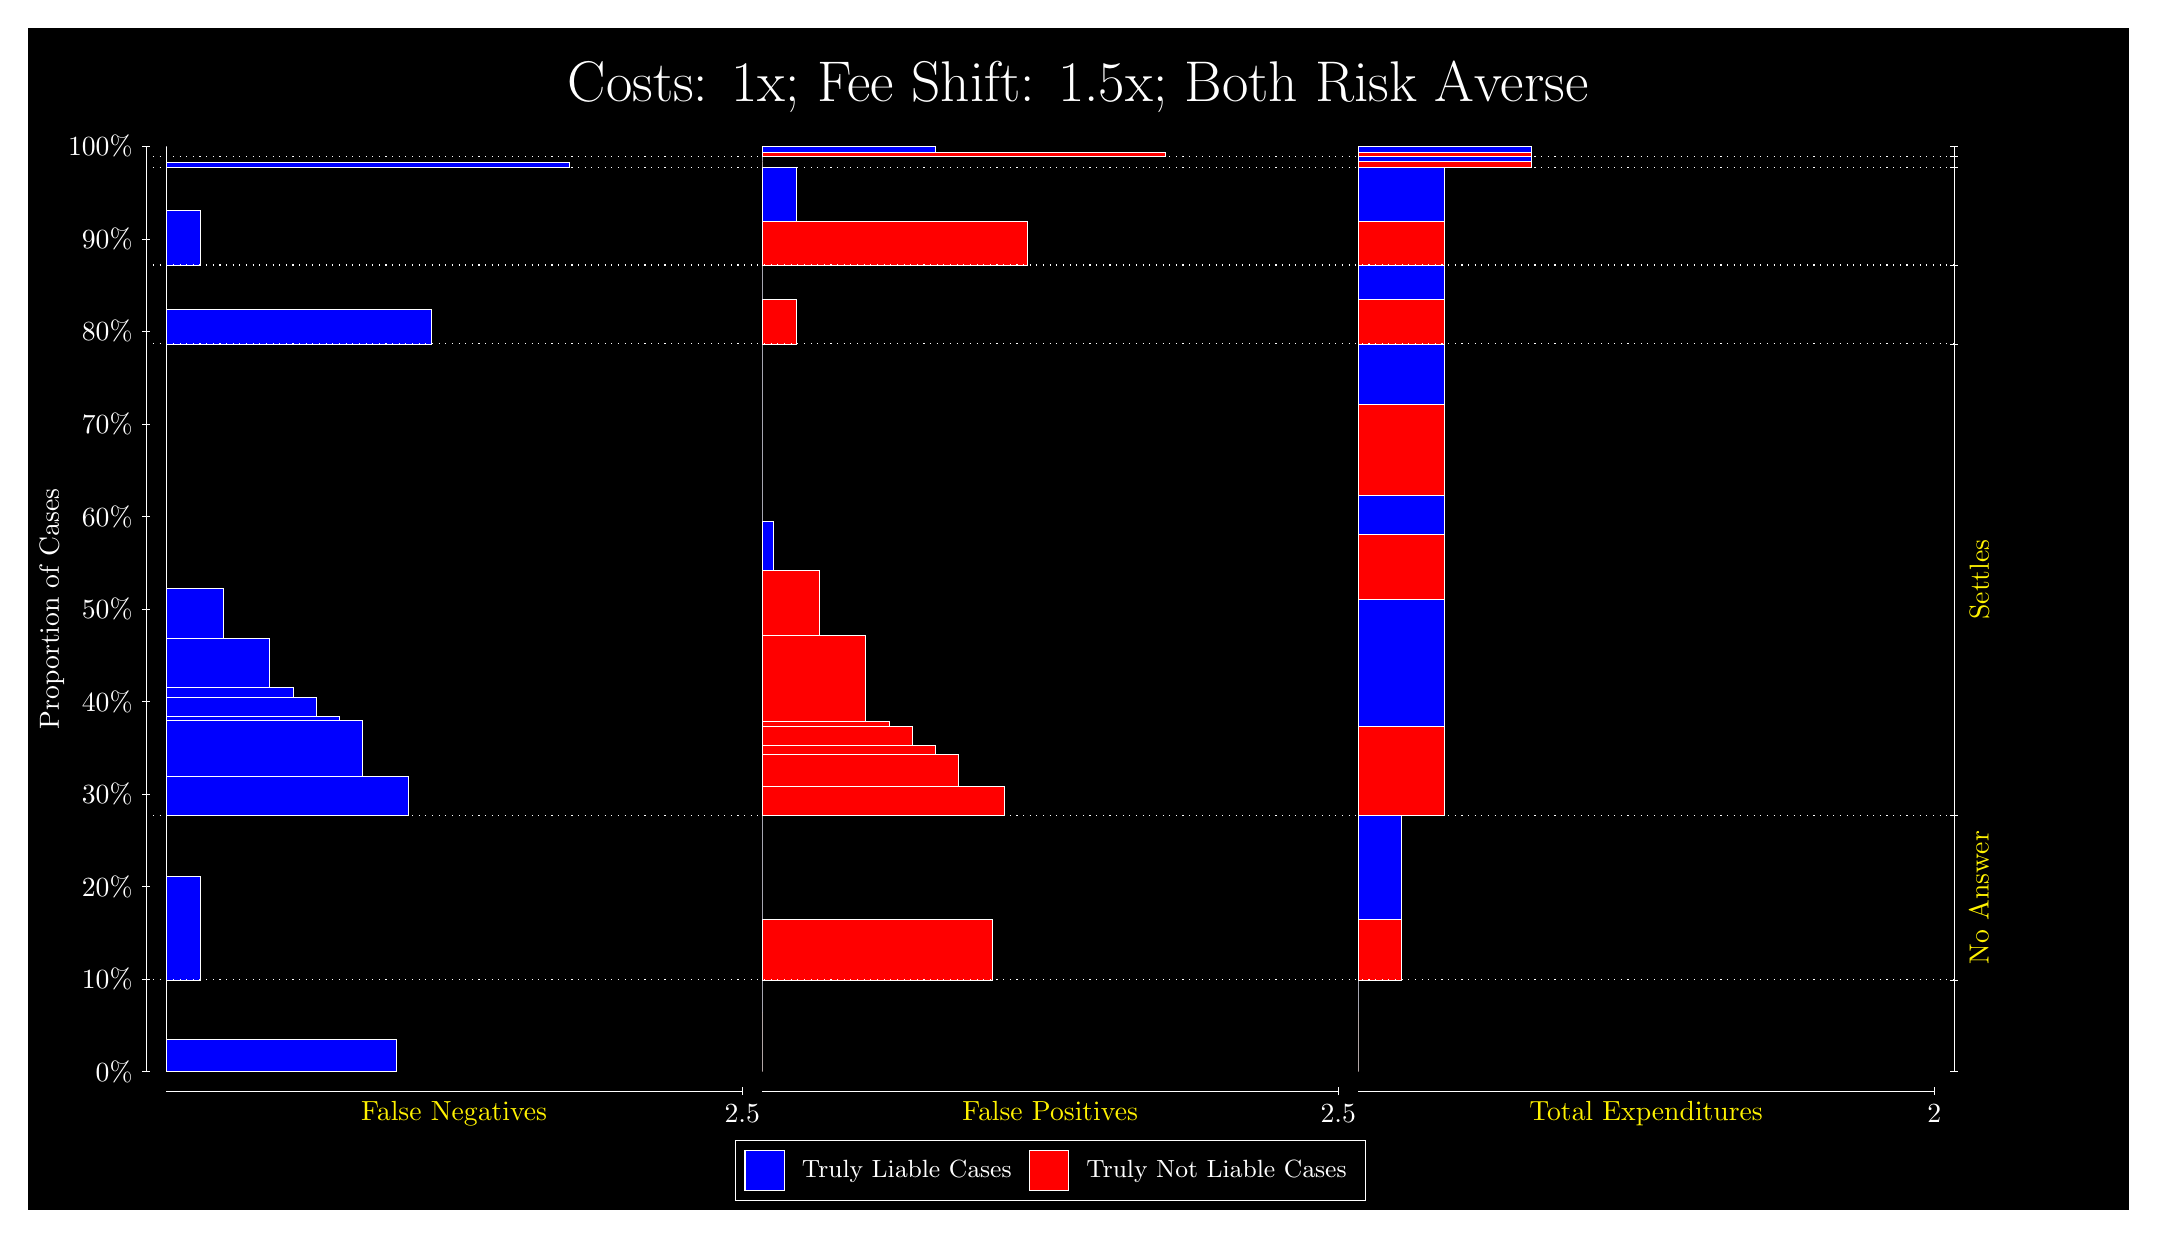
\begin{tikzpicture}
\draw[fill=black] (0,0) rectangle (26.667,15);
\draw[text=white] (0,13.5) rectangle (26.667,15) node[midway] {\huge Costs: 1x; Fee Shift: 1.5x; Both Risk Averse};
\draw[white, very thin] (1.5,1.75) -- (1.5,13.5);
\node[rotate=90, text=white, anchor=center] at (0.3, 7.625) {Proportion of Cases};
\draw[white, very thin] (1.45,1.75) -- (1.55,1.75);
\node[text=white, anchor=east] at (1.45, 1.75) {0\%};
\draw[white, very thin] (1.45,2.925) -- (1.55,2.925);
\node[text=white, anchor=east] at (1.45, 2.925) {10\%};
\draw[white, very thin] (1.45,4.1) -- (1.55,4.1);
\node[text=white, anchor=east] at (1.45, 4.1) {20\%};
\draw[white, very thin] (1.45,5.275) -- (1.55,5.275);
\node[text=white, anchor=east] at (1.45, 5.275) {30\%};
\draw[white, very thin] (1.45,6.45) -- (1.55,6.45);
\node[text=white, anchor=east] at (1.45, 6.45) {40\%};
\draw[white, very thin] (1.45,7.625) -- (1.55,7.625);
\node[text=white, anchor=east] at (1.45, 7.625) {50\%};
\draw[white, very thin] (1.45,8.8) -- (1.55,8.8);
\node[text=white, anchor=east] at (1.45, 8.8) {60\%};
\draw[white, very thin] (1.45,9.975) -- (1.55,9.975);
\node[text=white, anchor=east] at (1.45, 9.975) {70\%};
\draw[white, very thin] (1.45,11.15) -- (1.55,11.15);
\node[text=white, anchor=east] at (1.45, 11.15) {80\%};
\draw[white, very thin] (1.45,12.325) -- (1.55,12.325);
\node[text=white, anchor=east] at (1.45, 12.325) {90\%};
\draw[white, very thin] (1.45,13.5) -- (1.55,13.5);
\node[text=white, anchor=east] at (1.45, 13.5) {100\%};

\draw[white, very thin] (24.457,1.75) -- (24.457,13.5);
\draw[white, very thin] (24.407,1.75) -- (24.507,1.75);
\node[anchor=west] at (24.407, 1.75) {};
\draw[white, very thin] (24.407,2.9132) -- (24.507,2.9132);
\node[anchor=west] at (24.407, 2.9132) {};
\draw[white, very thin] (24.407,5.004) -- (24.507,5.004);
\node[anchor=west] at (24.407, 5.004) {};
\draw[white, very thin] (24.407,10.991) -- (24.507,10.991);
\node[anchor=west] at (24.407, 10.991) {};
\draw[white, very thin] (24.407,11.993) -- (24.507,11.993);
\node[anchor=west] at (24.407, 11.993) {};
\draw[white, very thin] (24.407,13.233) -- (24.507,13.233);
\node[anchor=west] at (24.407, 13.233) {};
\draw[white, very thin] (24.407,13.372) -- (24.507,13.372);
\node[anchor=west] at (24.407, 13.372) {};
\draw[white, very thin] (24.407,13.5) -- (24.507,13.5);
\node[anchor=west] at (24.407, 13.5) {};

\draw[white, very thin, fill=blue] (1.75,1.75) rectangle (4.6775,2.1599);
\draw[white, very thin, fill=red] (1.75,2.1599) rectangle (1.75,2.9133);
\draw[white, very thin, fill=blue] (1.75,2.9133) rectangle (2.1891,4.235);
\draw[white, very thin, fill=red] (1.75,4.235) rectangle (1.75,5.004);
\draw[white, very thin, fill=blue] (1.75,5.004) rectangle (4.8239,5.5002);
\draw[white, very thin, fill=blue] (1.75,5.5002) rectangle (4.2384,6.21);
\draw[white, very thin, fill=blue] (1.75,6.21) rectangle (3.9457,6.2663);
\draw[white, very thin, fill=blue] (1.75,6.2663) rectangle (3.6529,6.5057);
\draw[white, very thin, fill=blue] (1.75,6.5057) rectangle (3.3602,6.6299);
\draw[white, very thin, fill=blue] (1.75,6.6299) rectangle (3.0674,7.2576);
\draw[white, very thin, fill=blue] (1.75,7.2576) rectangle (2.4819,7.885);
\draw[white, very thin, fill=red] (1.75,7.885) rectangle (1.75,10.991);
\draw[white, very thin, fill=blue] (1.75,10.991) rectangle (5.1167,11.432);
\draw[white, very thin, fill=red] (1.75,11.432) rectangle (1.75,11.993);
\draw[white, very thin, fill=blue] (1.75,11.993) rectangle (2.1891,12.683);
\draw[white, very thin, fill=red] (1.75,12.683) rectangle (1.75,13.233);
\draw[white, very thin, fill=blue] (1.75,13.233) rectangle (6.8732,13.295);
\draw[white, very thin, fill=red] (1.75,13.295) rectangle (1.75,13.372);
\draw[white, very thin, fill=red] (1.75,13.372) rectangle (1.75,13.43);
\draw[white, very thin, fill=blue] (1.75,13.43) rectangle (1.75,13.5);
\draw[white, very thin, fill=red] (9.3189,1.75) rectangle (9.3189,2.5033);
\draw[white, very thin, fill=blue] (9.3189,2.5033) rectangle (9.3189,2.9133);
\draw[white, very thin, fill=red] (9.3189,2.9133) rectangle (12.246,3.6823);
\draw[white, very thin, fill=blue] (9.3189,3.6823) rectangle (9.3189,5.004);
\draw[white, very thin, fill=red] (9.3189,5.004) rectangle (12.393,5.3679);
\draw[white, very thin, fill=red] (9.3189,5.3679) rectangle (11.807,5.7811);
\draw[white, very thin, fill=red] (9.3189,5.7811) rectangle (11.515,5.8937);
\draw[white, very thin, fill=red] (9.3189,5.8937) rectangle (11.222,6.133);
\draw[white, very thin, fill=red] (9.3189,6.133) rectangle (10.929,6.1951);
\draw[white, very thin, fill=red] (9.3189,6.1951) rectangle (10.636,7.2864);
\draw[white, very thin, fill=red] (9.3189,7.2864) rectangle (10.051,8.1096);
\draw[white, very thin, fill=blue] (9.3189,8.1096) rectangle (9.4652,8.737);
\draw[white, very thin, fill=blue] (9.3189,8.737) rectangle (9.3189,10.991);
\draw[white, very thin, fill=red] (9.3189,10.991) rectangle (9.758,11.552);
\draw[white, very thin, fill=blue] (9.3189,11.552) rectangle (9.3189,11.993);
\draw[white, very thin, fill=red] (9.3189,11.993) rectangle (12.686,12.543);
\draw[white, very thin, fill=blue] (9.3189,12.543) rectangle (9.758,13.233);
\draw[white, very thin, fill=red] (9.3189,13.233) rectangle (9.3189,13.31);
\draw[white, very thin, fill=blue] (9.3189,13.31) rectangle (9.3189,13.372);
\draw[white, very thin, fill=red] (9.3189,13.372) rectangle (14.442,13.43);
\draw[white, very thin, fill=blue] (9.3189,13.43) rectangle (11.515,13.5);
\draw[white, very thin, fill=red] (16.888,1.75) rectangle (16.888,2.5033);
\draw[white, very thin, fill=blue] (16.888,2.5033) rectangle (16.888,2.9133);
\draw[white, very thin, fill=red] (16.888,2.9133) rectangle (17.437,3.6823);
\draw[white, very thin, fill=blue] (16.888,3.6823) rectangle (17.437,5.004);
\draw[white, very thin, fill=red] (16.888,5.004) rectangle (17.986,6.133);
\draw[white, very thin, fill=blue] (16.888,6.133) rectangle (17.986,7.7517);
\draw[white, very thin, fill=red] (16.888,7.7517) rectangle (17.986,8.5749);
\draw[white, very thin, fill=blue] (16.888,8.5749) rectangle (17.986,9.0711);
\draw[white, very thin, fill=red] (16.888,9.0711) rectangle (17.986,10.224);
\draw[white, very thin, fill=blue] (16.888,10.224) rectangle (17.986,10.991);
\draw[white, very thin, fill=red] (16.888,10.991) rectangle (17.986,11.552);
\draw[white, very thin, fill=blue] (16.888,11.552) rectangle (17.986,11.993);
\draw[white, very thin, fill=red] (16.888,11.993) rectangle (17.986,12.543);
\draw[white, very thin, fill=blue] (16.888,12.543) rectangle (17.986,13.233);
\draw[white, very thin, fill=red] (16.888,13.233) rectangle (19.083,13.31);
\draw[white, very thin, fill=blue] (16.888,13.31) rectangle (19.083,13.372);
\draw[white, very thin, fill=red] (16.888,13.372) rectangle (19.083,13.43);
\draw[white, very thin, fill=blue] (16.888,13.43) rectangle (19.083,13.5);
\draw[white, dotted] (1.5,2.9133) -- (24.457,2.9133);
\draw[white, dotted] (1.5,5.004) -- (24.457,5.004);
\draw[white, dotted] (1.5,10.991) -- (24.457,10.991);
\draw[white, dotted] (1.5,11.993) -- (24.457,11.993);
\draw[white, dotted] (1.5,13.233) -- (24.457,13.233);
\draw[white, dotted] (1.5,13.372) -- (24.457,13.372);
\draw[white, very thin] (1.75,1.5) -- (9.0689,1.5);
\node[text=yellow, anchor=north] at (5.4094, 1.5) {False Negatives};
\draw[white, very thin] (9.0689,1.45) -- (9.0689,1.55);
\node[text=white, anchor=north] at (9.0689, 1.45) {2.5};

\draw[white, very thin] (9.3189,1.5) -- (16.638,1.5);
\node[text=yellow, anchor=north] at (12.978, 1.5) {False Positives};
\draw[white, very thin] (16.638,1.45) -- (16.638,1.55);
\node[text=white, anchor=north] at (16.638, 1.45) {2.5};

\draw[white, very thin] (16.888,1.5) -- (24.207,1.5);
\node[text=yellow, anchor=north] at (20.547, 1.5) {Total Expenditures};
\draw[white, very thin] (24.207,1.45) -- (24.207,1.55);
\node[text=white, anchor=north] at (24.207, 1.45) {2};


\node[text=yellow, centered, rotate=90] at (24.777, 3.9586) {No Answer};
\node[text=yellow, centered, rotate=90] at (24.777, 7.9973) {Settles};





\draw (12.978300999999998,1.5) node[draw=none] (baseCoordinate) {};
\begin{scope}[align=center]
        \matrix[scale=0.5, draw=white, below=0.5cm of baseCoordinate, nodes={draw}, column sep=0.1cm]{
            \node[rectangle, draw, minimum width=0.5cm, minimum height=0.5cm, fill=blue] {}; &
            \node[draw=none, font=\small, text=white] (B) {Truly Liable Cases}; &
            \node[rectangle, draw, minimum width=0.5cm, minimum height=0.5cm, fill=red] {}; &
            \node[draw=none, font=\small, text=white] (B) {Truly Not Liable Cases}; \\
            };
\end{scope}

\end{tikzpicture}
\end{document}